\section{Machine Learning and Deep Learning Models for Sentiment Analysis}
\label{sec:ML_DL_Models}

\subsection{Introduction}
In this section, we present and discuss the machine learning and deep learning models implemented in this project, focusing on their structure, functionality, and contributions to the problem of Twitter sentiment analysis. These models fall within the supervised learning paradigm, with some lexicon-based approaches also explored, and are specifically chosen to address the challenges inherent in classifying sentiment from short, informal, and often noisy text data from Twitter.

We begin with an exploration of traditional Machine Learning (ML) models like Support Vector Machines (SVMs) using Bag-of-Words (BoW) and TF-IDF features. We then discuss lexicon-based approaches such as VADER and TextBlob. Following this, we delve into several neural network architectures, including Feedforward Neural Networks (FNNs), Convolutional Neural Networks (CNNs) adapted for text, and various Recurrent Neural Networks (RNNs) like Long Short-Term Memory (LSTM), Gated Recurrent Units (GRU), and Bidirectional LSTMs (Bi-LSTMs). Finally, we cover the powerful transformer-based model, BERT.

Each model leverages unique mechanisms to process and learn from textual data, enabling accurate classification of tweet sentiment. Furthermore, we describe the text pre-processing steps, feature extraction techniques, and hyperparameter tuning strategies employed to optimize these models for enhanced performance. The discussion also touches upon how data characteristics unique to Twitter are handled.

Finally, we outline the evaluation metrics and hyperparameters used to assess the models’ effectiveness. These metrics provide a comprehensive understanding of the models’ predictive accuracy, robustness, and suitability for the sentiment classification task at hand.

\subsection{Traditional Machine Learning Approaches}

\subsubsection{Support Vector Machines (SVM)}
Support Vector Machines are supervised learning models renowned for their effectiveness in classification tasks, particularly in high-dimensional spaces. The core idea of SVM is to find an optimal hyperplane that best separates data points belonging to different classes in the feature space. For non-linearly separable data, SVMs can use a "kernel trick" (e.g., polynomial, radial basis function (RBF) kernels) to map data into a higher-dimensional space where a linear separation becomes possible.

\begin{figure} [h!]
    \centering
    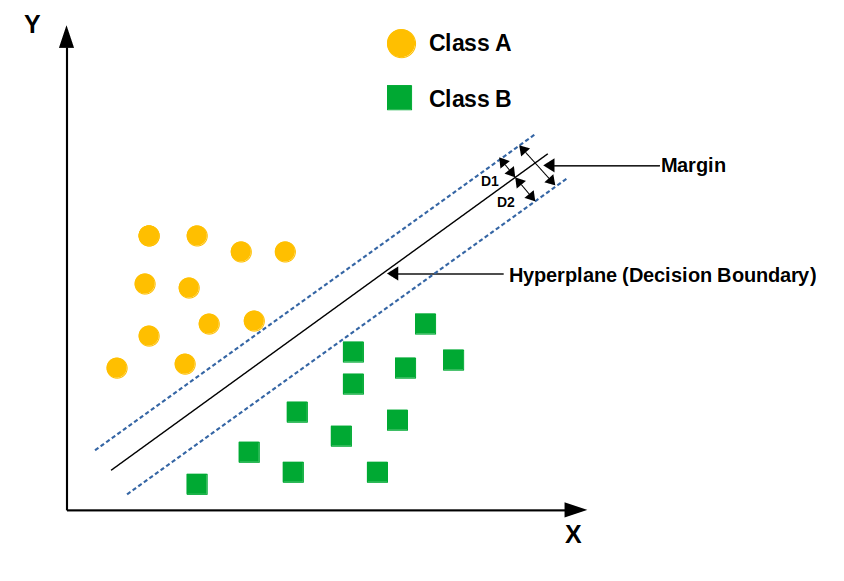
\includegraphics[width=0.75\linewidth]{images/svm_arch.png}
    \caption{SVM Structure}
    \label{fig:enter-label}
\end{figure}

For Twitter sentiment analysis, SVMs are typically used with text features extracted using methods like:

\begin{itemize}
    \item Bag-of-Words (BoW): This approach represents text by the occurrence of words within it, disregarding grammar and word order but keeping multiplicity. Each tweet is converted into a vector where each dimension corresponds to a word in the vocabulary, and the value can be the count of the word or a binary indicator of its presence.
    \item Term Frequency-Inverse Document Frequency (TF-IDF): TF-IDF is a numerical statistic that reflects how important a word is to a document (a tweet, in this case) in a collection or corpus. It increases proportionally to the number of times a word appears in the document but is offset by the frequency of the word in the corpus. This helps to give more weight to words that are frequent in a tweet but not frequent across all tweets.
\end{itemize}

SVMs trained on BoW or TF-IDF features have demonstrated strong performance in many text classification tasks, including sentiment analysis, by effectively navigating the sparsity and high dimensionality of such data.

\subsection{Lexicon-Based Approaches}
Lexicon-based approaches classify sentiment based on the semantic orientation of words and phrases present in the text. They rely on a sentiment lexicon, which is a dictionary of words pre-annotated with their sentiment scores (e.g., positive, negative, neutral) and sometimes intensity.

\subsubsection{VADER (Valence Aware Dictionary and Sentiment Reasoner)}
VADER is a lexicon and rule-based sentiment analysis tool specifically attuned to sentiments expressed in social media. It considers lexical features common in microblogging, such as emoticons, slang, acronyms, and degree modifiers (e.g., "very," "extremely"). VADER produces a sentiment score (compound score) that indicates both the polarity (positive/negative) and intensity of the sentiment. It is particularly useful for analyzing Twitter data due to its focus on social media language and its ability to perform well without training data.

\subsubsection{TextBlob}
TextBlob is a Python library providing a simple API for common NLP tasks, including sentiment analysis. Its sentiment analysis functionality is built upon a lexicon (often based on WordNet) and a set of rules to determine sentiment polarity (ranging from -1 to 1) and subjectivity (ranging from 0 to 1). While easy to use, its general-purpose lexicon might be less effective on nuanced or domain-specific Twitter language compared to VADER unless customized.

\subsection{Feedforward Neural Networks (FNN)}
A Feedforward Neural Network (FNN), also known as a Multi-Layer Perceptron (MLP), is one of the simplest forms of artificial neural networks. It is designed to approximate functions by mapping input data to output labels through a series of hidden layers. FNNs process information in one direction—from the input layer, through the hidden layers, to the output layer—without forming cycles or loops.

\begin{figure}[h!]
    \centering
    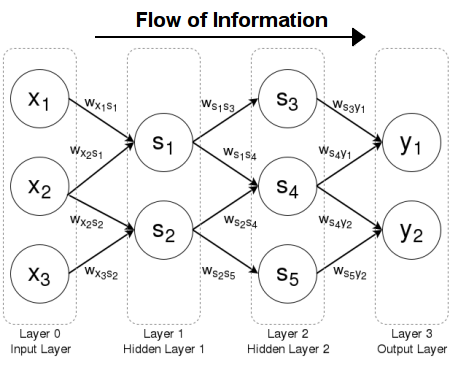
\includegraphics[width=0.8\linewidth]{images/fnn-str.png}
    \caption{Structure of a Feedforward Neural Network}
    \label{fig:feedforward_structure}
\end{figure}

Each neuron in an FNN applies a weighted sum to its inputs, adds a bias, and passes the result through an activation function:
$$
y = f\left(\sum_{i=1}^{n} w_i x_i + b\right)
$$
where (y) is the output, (x\_i) are inputs, (w\_i) are weights, (b) is bias, and (f) is an activation function (e.g., ReLU, Sigmoid).

An FNN consists of:

\begin{itemize}
    \item Input Layer: Receives input features. For text, these features are often word embeddings (dense vector representations of words) or TF-IDF vectors.
    \item Hidden Layers: Perform transformations using weights, biases, and activation functions. The depth and width of these layers determine the model's capacity.
    \item Output Layer: Produces predictions. For sentiment classification (e.g., positive, negative, neutral), a Softmax activation function is typically used to output class probabilities.
\end{itemize}


\begin{figure}[H]
    \centering
    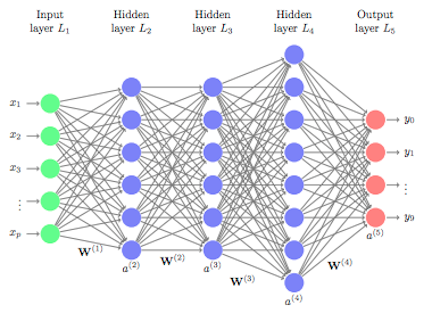
\includegraphics[width=1\linewidth]{images/feedforward_workflow.png}
    \caption{Workflow of a Feedforward Neural Network}
    \label{fig:feedforward_workflow}
\end{figure}

The workflow involves forward propagation (calculating output), loss calculation (measuring error), backpropagation (calculating gradients), and optimization (updating weights).

For text classification, FNNs can be effective when used with appropriate input representations like pre-trained word embeddings (e.g., Word2Vec, GloVe, FastText) or TF-IDF vectors. While they don't inherently capture sequential information like RNNs or local contextual patterns like CNNs for text, they can serve as strong classifiers on aggregated or transformed text features.

\subsection{Convolutional Neural Networks (CNN) for Text}
While traditional Neural Networks like FNNs can struggle with the high dimensionality and local structure of raw text, Convolutional Neural Networks (CNNs), originally designed for image processing, have been successfully adapted for text classification tasks. Instead of applying 2D convolutions to image pixels, 1D convolutions are applied over sequences of word embeddings.

\begin{figure}[h!]
    \centering
    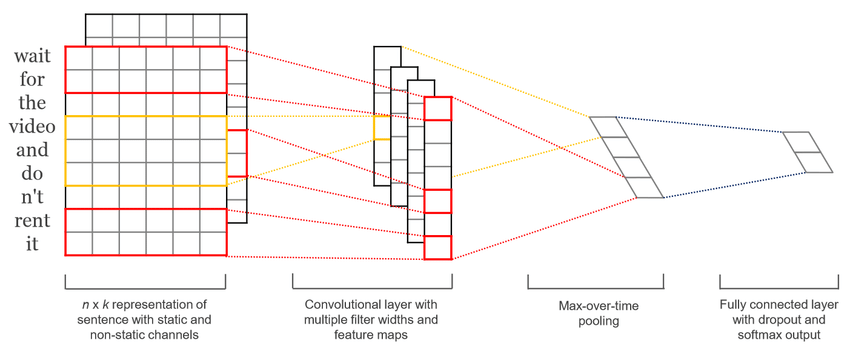
\includegraphics[width=0.75\linewidth]{images/cnn-struture.png}
    \caption{CNN Struture (Text Example}
    \label{fig:enter-label}
\end{figure}

In this context:

\begin{itemize}
    \item Input Representation: Tweets are first converted into a matrix where each row represents a word and columns represent the dimensions of its word embedding (e.g., from Word2Vec, GloVe, or learned during training).
    \item Convolutional Layer: 1D filters (kernels) of different lengths (e.g., spanning 2, 3, or 4 words at a time, akin to n-grams) slide across the sequence of word embeddings. Each convolution operation produces a feature. The idea is that these filters learn to detect meaningful patterns or n-grams relevant to sentiment (e.g., "very good," "not bad").
    \item Activation Function: A non-linear activation function like ReLU is applied to the output of the convolutions.
    \item Pooling Layer: A 1D max-over-time pooling operation is typically applied to the feature maps generated by the convolutional layer. This takes the maximum value over the time (sequence) dimension for each filter, effectively capturing the most salient feature detected by that filter across the entire tweet. This also results in a fixed-size output vector, regardless of the input tweet length.
    \item Fully Connected Layer: The pooled features from various filters are concatenated and fed into one or more fully connected layers, culminating in an output layer (e.g., with Softmax activation) for sentiment classification.
\end{itemize}
CNNs for text are effective at capturing local contextual information and hierarchical features from text data. They are computationally less expensive than some RNN variants and can be very powerful, especially when combined with pre-trained word embeddings.


\subsection{Recurrent Neural Networks (RNN)}
Recurrent Neural Networks are specifically designed for processing sequential data like text, where the order of elements (words) is crucial. Unlike FNNs, RNNs have connections that form directed cycles, allowing them to maintain an internal state or "memory" of past information while processing a sequence.

\subsubsection{Long Short-Term Memory (LSTM)}
Standard RNNs suffer from the vanishing gradient problem, making it difficult for them to learn long-range dependencies in sequences. LSTMs address this issue through a more complex recurrent unit containing three "gates":

\begin{itemize}
    \item Input Gate: Controls how much of the new input is let into the memory cell.
    \item Forget Gate: Controls how much of the existing memory cell content is forgotten.
    \item Output Gate: Controls how much of the memory cell content is passed to the output and the next hidden state.
\end{itemize}

These gates allow LSTMs to selectively remember or forget information over long sequences, making them highly effective for tasks like sentiment analysis where context from earlier parts of a sentence (or tweet) can influence the overall sentiment.

\subsubsection{Gated Recurrent Units (GRU)}
GRUs are a variation of LSTMs that simplify the gating mechanism. They have two gates:

\begin{itemize}
    \item Reset Gate: Determines how to combine the new input with the previous memory.
    \item Update Gate: Determines how much of the previous memory to keep.
\end{itemize}

GRUs often achieve performance comparable to LSTMs on many tasks but with fewer parameters, potentially leading to faster training and less overfitting on smaller datasets.

\subsubsection{Bidirectional LSTMs (Bi-LSTM)}
Standard LSTMs (and GRUs) process sequences in one direction (e.g., from left to right). However, the sentiment of a tweet can depend on context from both preceding and succeeding words. Bidirectional LSTMs address this by using two separate LSTM layers: one processes the input sequence from start to end (forward layer), and the other processes it from end to start (backward layer). The outputs from both layers at each time step are typically concatenated (or combined in other ways) before being passed to the next layer. This allows the model to have a more complete understanding of the context of each word in the tweet. Bi-LSTMs often outperform unidirectional LSTMs in sentiment analysis tasks.

\subsection{BERT (Bidirectional Encoder Representations from Transformers)}
BERT represents a significant advancement in NLP, leveraging the Transformer architecture, which relies heavily on a mechanism called self-attention. Unlike RNNs that process words sequentially, Transformers process all words in a sequence simultaneously, allowing the model to weigh the importance of different words when representing each word in its context.

Key aspects of BERT include:

\begin{itemize}
    \item Pre-training: BERT is pre-trained on massive amounts of unlabeled text data (like Wikipedia and BooksCorpus) using two unsupervised tasks: Masked Language Model (MLM) and Next Sentence Prediction (NSP). This allows BERT to learn rich, deep bidirectional representations of language.
    \item Bidirectionality: Unlike earlier models like GPT (which were unidirectional), BERT's self-attention mechanism allows it to consider both left and right context for every word in a sequence from the very beginning of pre-training.
    \item Fine-tuning: After pre-training, BERT can be fine-tuned for various downstream NLP tasks, including sentiment analysis, by adding a small task-specific output layer and training on labeled data. For sentiment classification, a classification layer is typically added on top of the [CLS] token's output representation from BERT.
    \item 
\end{itemize}
BERT and its variants (e.g., RoBERTa, ALBERT, DistilBERT, and domain-specific versions like BERTweet for Twitter data) have achieved state-of-the-art results on many NLP benchmarks. For Twitter sentiment analysis, fine-tuning a pre-trained BERT model can yield very strong performance by leveraging its robust understanding of language nuances.

\subsection{Text Pre-processing, Data Augmentation for Text and Hyperparameter Tuning}

To enhance the performance and generalization of the sentiment analysis models, this study employs several techniques.

\subsubsection{Text Pre-processing}
Twitter data is notoriously noisy, containing slang, misspellings, abbreviations, URLs, mentions (@username), hashtags (\#topic), and emoticons. Effective pre-processing is crucial:

\begin{itemize}
    \item \textbf{Cleaning}: Removing URLs, mentions, special characters (while retaining sentiment-bearing ones like emoticons or punctuation like '!'), and HTML tags.
    \item \textbf{Normalization}: Converting text to lowercase, correcting common misspellings or slang (e.g., "u" to "you"), expanding contractions (e.g., "can't" to "cannot").
    \item \textbf{Tokenization}: Splitting tweets into individual words or sub-word units.
    \item \textbf{Stop Word Removal}: Optionally removing common words (e.g., "the," "is," "in") that may not carry significant sentiment, although this can sometimes be detrimental if not done carefully (e.g., "not" is a stop word but crucial for sentiment).
    \item \textbf{Lemmatization/Stemming}: Reducing words to their root form (e.g., "running" to "run"). Lemmatization is generally preferred as it results in actual words.
\end{itemize}

\subsubsection{Data Augmentation for Text}
Data augmentation for text aims to artificially increase the diversity of the training dataset. While not as straightforward as image augmentation, common techniques include:

\begin{itemize}
    \item \textbf{Synonym Replacement}: Randomly replacing words with their synonyms (e.g., using WordNet).
    \item \textbf{Random Insertion}: Inserting random synonyms of words at random positions.
    \item \textbf{Random Deletion}: Randomly deleting words from a sentence.
    \item \textbf{Back-Translation}: Translating a sentence to another language and then back to the original, which can create paraphrased versions.
\end{itemize}

\subsubsection{Hyperparameter Tuning}
Hyperparameter tuning involves systematically optimizing the parameters that govern the training process and architecture of the models. 

By integrating thorough text pre-processing and hyperparameter tuning into the modeling workflow, the implemented models are better equipped to handle the challenges of Twitter sentiment analysis, yielding improved accuracy and robustness in their predictions.

\subsection{Model Evaluation: Confusion Matrix and Classification Metrics}

The evaluation of the sentiment analysis models will be carried out using the confusion matrix, which provides a detailed view of the model’s correct and incorrect predictions for each sentiment class (e.g., positive, negative, neutral). In addition, classification metrics including \textit{accuracy}, \textit{precision}, \textit{recall}, and \textit{F1-score} will be calculated. These metrics are essential for assessing the effectiveness of the model in differentiating between various sentiment types.

\subsubsection{Confusion Matrix}

A confusion matrix is a table that indicates the mistakes and successes of your model, comparing to the expected result. The layout of a confusion matrix is present on the next figure. We will utilize the confusion\_matrix function from scikit-learn.

\begin{figure}[h!]
    \centering
    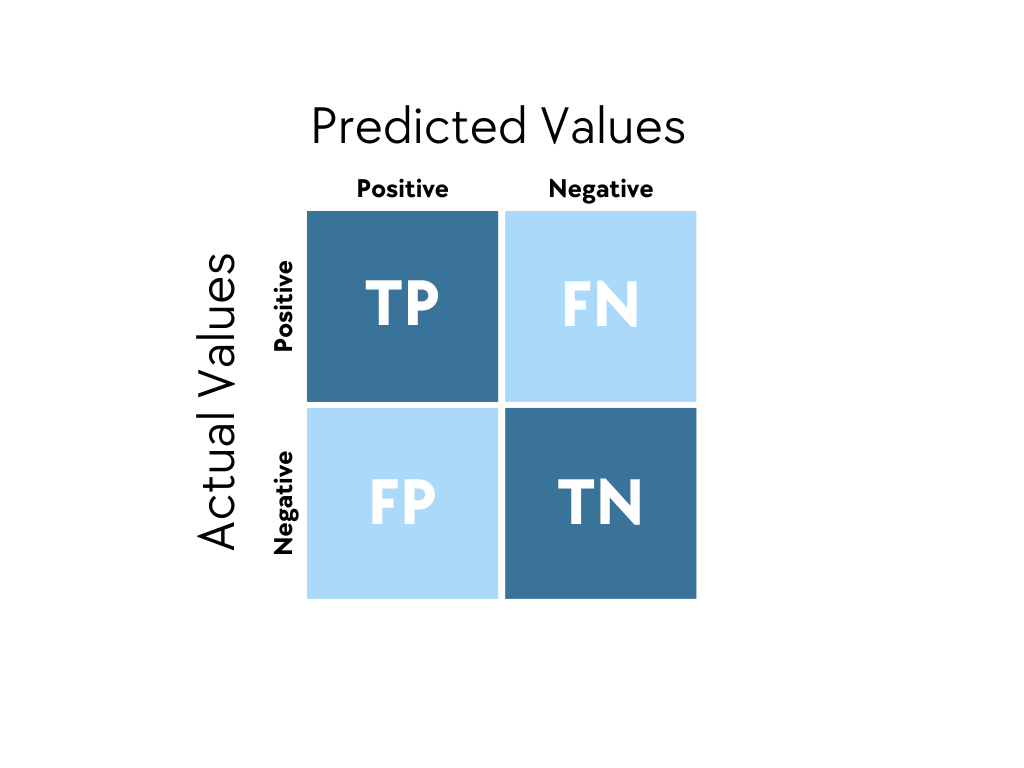
\includegraphics[width=1\linewidth]{images/confusion-matrix.png}
    \caption{Confusion Matrix}
    \label{fig:confusion_matrix}
\end{figure}

\subsubsection{Precision}
Precision measures the ratio of true positive predictions to the total number of positive predictions made by the model. It answers the question: "Of all tweets predicted as positive, how many were actually positive?"
$$Precision=\frac{True Positives (TP)}{True Positives (TP)+False Positives (FP)}$$

\subsubsection{Recall (Sensitivity)}
Recall (or sensitivity, or True Positive Rate) gauges the model’s ability to correctly identify all relevant instances from the total number of actual positive instances in the dataset. It answers: "Of all actual positive tweets, how many did the model correctly predict as positive?"
$$Recall=\frac{True Positives (TP)}{True Positives (TP)+False Negatives (FN)}$$

\subsubsection{F1-Score}
The F1-score is the harmonic mean of precision and recall, providing a balanced assessment of a model’s performance, especially useful when class distributions are imbalanced.
$$F1Score=2 \times \frac{Precision \times Recall}{Precision+Recall}$$

\subsubsection{Accuracy}
Accuracy is the proportion of correct predictions (both true positives and true negatives for binary, or sum of correct predictions across all classes for multi-class) to the total number of predictions made. It represents the overall correctness of the model's predictions.
$$Accuracy= \frac{\text{Number of Correct Predictions}}{\text{Total Number of Predictions}}$$


\subsubsection{Training Loss}
Training loss quantifies how well the model fits the training data by calculating the difference between predicted and actual values using a loss function (e.g., cross-entropy for classification). A lower loss generally indicates better model fit. The goal during training is to minimize this loss, though monitoring validation loss is crucial to prevent overfitting.